\chapter{Constructing the Borel and Lebesgue measure}
It's very difficult to define in one breath a measure
on the Borel space $\SB(\RR^n)$.
It is easier if we define a weaker notion first.
There are two such weaker notions that we will define:
\begin{itemize}
	\ii A \textbf{pre-measure}:
	satisfies the axioms of a measure,
	but defined on \emph{fewer} sets than a measure:
	they'll be defined on an ``algebra''
	rather than the full-fledged ``$\sigma$-algebra''.

	\ii An \textbf{outer measure}:
	defined on $2^\Omega$ but satisfies weaker axioms.
\end{itemize}
It will turn out that pre-measures yield outer measures,
and outer measures yield measures.


\section{Pre-measures}
\prototype{Let $\Omega = \RR^2$. Then we take $\SA_0$ generated by rectangles,
	with $\mu_0$ the usual area.}
The way to define a pre-measure is to weaken
the $\sigma$-algebra to an algebra.
\begin{definition}
	Let $\Omega$ be a set.
	We define notions of an \vocab{algebra},
	which is the same as $\sigma$-algebra except
	with ``countable'' replaced by finite everywhere.

	That is: an algebra $\SA_0$ on $\Omega$ is a
	nonempty subset of $2^\Omega$,
	which is closed under complement and \emph{finite} union.
	The smallest algebra containing a subset $\SF \subseteq 2^\Omega$
	is the \vocab{algebra generated by $\SF$}.
\end{definition}
In practice, we will basically always use generation for algebras.
\begin{example}
	When $\Omega = \RR^n$,
	we can let $\mathcal{L}_0$ be the algebra generated by
	$[a_1, b_1] \times \dots \times [a_n, b_n]$.
	A typical element might look like:
	\begin{center}
	\begin{asy}
		size(5cm);
		filldraw( (0,0)--(9,0)--(9,2)--(6,2)--(6,5)--(0,5)--cycle,
			opacity(0.1)+lightcyan, heavycyan );
		filldraw( (7,3)--(12,3)--(12,6)--(7,6)--cycle,
			opacity(0.1)+lightcyan, heavycyan );
	\end{asy}
	\end{center}
	Unsurprisingly, since we have \emph{finitely} many
	rectangles and their complements involved,
	in this case we actually \emph{can}
	unambiguously assign an area, and will do so soon.
\end{example}

\begin{definition}
	A \vocab{pre-measure} $\mu_0$ on a algebra $\SA_0$
	is a function $\mu_0 \colon \SA_0 \to [0, +\infty]$
	which satisfies the axioms
	\begin{itemize}
		\ii $\mu_0(\varnothing) = 0$, and
		\ii \textbf{Countable additivity}:
		if $A_1$, $A_2$, \dots are disjoint sets in $\SA_0$
		and \emph{moreover} the disjoint union $\bigsqcup A_i$
		is contained in $\SA_0$ (not guaranteed by algebra axioms!),
		then
		\[ \mu_0\left( \bigsqcup_n A_n \right) = \sum_n \mu_0(A_n). \]
	\end{itemize}
\end{definition}

\begin{example}
	[The pre-measure on $\RR^n$]
	Let $\Omega = \RR^2$.
	Then, let $\mathcal{L}_0$ be the algebra generated by rectangles
	$[a_1, a_2] \times [b_1, b_2]$.
	We then let
	\[ \mu_0\left( [a_1, a_2] \times [b_1, b_2] \right)
	= (a_2-a_1)(b_2-b_1) \]
	the area of the rectangle.
	As elements of $\mathcal{L}_0$ are simply \emph{finite} unions
	of rectangles and their complements (picture drawn earlier),
	it's not difficult to extend this to a pre-measure $\lambda_0$
	which behaves as you expect --- although we won't do this.
\end{example}

Since we are sweeping something under the rug that
turns out to be conceptually important,
I'll go ahead and blue-box it.
\begin{proposition}
	[Geometry sanity check that we won't prove]
	\label{prop:lebesgue_rectangle}
	For $\Omega = \RR^n$ and $\mathcal{L}_0$
	the algebra generated by rectangular prisms,
	one can define a pre-measure $\lambda_0$ on $\mathcal{L}_0$.
\end{proposition}
From this point forwards, we will basically do
almost no geometry\footnote{White lie.
	Technically, we will use one more fact:
	that open sets of $\RR^n$ can be covered by countably
	infinitely many rectangles,
	as in \Cref{exer:cubes_vs_open}.
	This step doesn't involve any area assignments, though.}
whatsoever in defining the measure $\SB(\RR^n)$,
and only use set theory to extend our measure.
So, \Cref{prop:lebesgue_rectangle} is the only sentry
which checks to make sure that our ``initial definition'' is sane.

To put the point another way,
suppose an \textbf{insane scientist}\footnote{Because
	``mad scientists'' are overrated.}
tried to define a notion
of area in which every rectangle had area $1$.
Intuitively, this shouldn't be possible:
every rectangle can be dissected into two halves
and we ought to have $1+1 \ne 1$.
However, the only thing that would stop them is that they couldn't
extend their pre-measure on the algebra $\mathcal{L}_0$.
If they somehow got past that barrier and got a pre-measure,
nothing in the rest of the section would prevent them
from getting an entire \emph{bona fide} measure with this property.
Thus, in our construction of the Lebesgue measure,
most of the geometric work is captured in the (omitted) proof
of \Cref{prop:lebesgue_rectangle}.

\section{Outer measures}
\prototype{Keep taking $\Omega = \RR^2$; see the picture to follow.}
The other way to weaken a measure is to relax the countable additivity,
and this yields the following:
\begin{definition}
	An \vocab{outer measure} $\mu^\ast$ on a set $\Omega$
	is a function $\mu^\ast \colon 2^\Omega \to [0, +\infty]$
	satisfying the following axioms:
	\begin{itemize}
		\ii $\mu^\ast(\varnothing) = 0$;
		\ii if $E \subseteq F$ and $E,F \in 2^{\Omega}$
		then $\mu^\ast(E) \le \mu^\ast(F)$;
		\ii for any subsets $E_1$, $E_2$, \dots of $\Omega$ we have
		\[ \mu^\ast \left( \bigcup_n E_n \right)
			\le \sum_n \mu^\ast(E_n). \]
	\end{itemize}
	(I don't really like the word ``outer measure'',
	since I think it is a bit of a misnomer:
	I would rather call it ``fake measure'',
	since it's not a measure either.)
\end{definition}

The reason for the name ``outer measure''
is that you almost always obtain outer measures
by approximating them from ``outside'' sets.
Officially, the result is often stated as follows
(as \Cref{pr:construct_outer_measure}).
\begin{quote}
	For a set $\Omega$, let $\mathcal{E}$ be \emph{any} subset of $2^{\Omega}$
	and let $\rho \colon \mathcal{E} \to [0,+\infty]$ be \emph{any} function.
	Then
	\[ \mu^\ast(E) = \inf \left\{ \sum_{n=1}^\infty \rho(E_n) \mid
		E_n \in \mathcal{E}, \;
		E \subseteq \bigcup_{n=1}^\infty E_n \right\} \]
	is an outer measure.
\end{quote}

However, I think the above theorem is basically always
wrong to use in practice, because it is \emph{way too general}.
As I warned with the insane scientist,
we really do want some sort of sanity conditions on $\rho$:
otherwise, if we apply the above result as stated,
there is no guarantee that $\mu^\ast$ will
be compatible with $\rho$ in any way.

%So, the recipe so far goes like:
%define an algebra $\SA_0$ generated by some sets with
%``known'' measure (like rectangles) and checking it extends well,
%then get an outer measure from it.
%In the next section, we will then see every outer measure gives a true measure.

So, I think it is really better to apply the theorem to pre-measures $\mu_0$
for which one \emph{does} have some sort of guarantee
that the resulting $\mu^\ast$ is compatible with $\mu_0$.
In practice, this is always how we will want to construct our outer measures.
\begin{theorem}
	[Constructing outer measures from pre-measures]
	\label{thm:construct_outer}
	Let $\mu_0$ be a pre-measure on an algebra $\SA_0$ on a set $\Omega$.
	\begin{enumerate}[(a)]
		\ii The map $\mu^\ast \colon 2^\Omega \to [0,+\infty]$ defined by
		\[ \mu^\ast(E) = \inf \left\{ \sum_{n=1}^\infty \mu_0(A_n) \mid
			A_n \in \SA_0, \; E \subseteq \bigcup_{n=1}^\infty A_n \right\} \]
		is an outer measure.
		\ii Moreover, this measure agrees with $\mu_0$ on sets in $\SA_0$.
	\end{enumerate}
\end{theorem}
Intuitively, what is going on is that
$\mu^\ast(A)$ is the infimum of coverings of $A$ by
countable unions of elements in $\SA_0$.
Part (b) is the first half of the compatibility condition I promised;
the other half appears later as \Cref{prop:cm_compatible}.

\begin{proof}
	[Proof of \Cref{thm:construct_outer}]
	As alluded to already, part (a)
	is a special case of \Cref{pr:construct_outer_measure}
	(and proving it in this generality is actually easier,
	because you won't be distracted by unnecessary properties).

	We now check (b), that $\mu^\ast(A) = \mu_0(A)$ for $A \in \SA_0$.
	One bound is quick:
	\begin{ques}
		Show that $\mu^\ast(A) \le \mu_0(A)$.
	\end{ques}
	For the reverse, suppose that $A \subseteq \bigcup_n A_n$.
	Then, define the sets
	\begin{align*}
		B_1 &= A \cap A_1 \\
		B_2 &= (A \cap A_2) \setminus B_1 \\
		B_3 &= (A \cap A_3) \setminus B_2 \\
		&\vdotswithin=
	\end{align*}
	and so on.
	Then the $B_n$ are disjoint elements of $\SA_0$ with $B_n \subset A_n$,
	and we have rigged the definition so that $\bigsqcup_n B_n = A$.
	Thus by definition of pre-measure,
	\[ \mu_0(A) = \sum_n \mu_0(B_n) \le \sum_n \mu_0(A_n) \]
	as desired.
\end{proof}

\begin{example}
	Let $\Omega = \RR^2$ and $\lambda_0$ the pre-measure from before.
	Then $\lambda^\ast(A)$ is, intuitively,
	the infimum of coverings of the set $A$ by rectangles.
	Here is a picture you might use to imagine the
	situation with $A$ being the unit disk.
	\missingfigure{circles covered by rectangles}
\end{example}



\section{Carath\'{e}odory extension for outer measures}
We will now take any outer measure and turn it into a proper measure.
To do this, we first need to specify the $\sigma$-algebra
on which we will define the measure.

\begin{definition}
	Let $\mu^\ast$ be an outer measure.
	We say a set $A$ is \vocab{Carath\'{e}odory measurable with respect
	to $\mu^\ast$}, or just \vocab{$\mu^\ast$-measurable},
	if the following condition holds:
	for any set $E \in 2^{\Omega}$,
	\[ \mu^\ast(E) = \mu^\ast(E \cap A) + \mu^\ast(E \setminus A). \]
\end{definition}
This definition is hard to motivate, but turns out to be the right one.
One way to motivate is this:
it turns out that in $\RR^n$,
it will be equivalent to a reasonable geometric condition
(which I will state in \Cref{prop:lebesgue_geo}),
but since that geometric definition requires information about $\RR^n$ itself,
this is the ``right'' generalization for general measure spaces.

Since our goal was to extend our $\SA_0$,
we had better make sure this definition
lets us measure the initial sets that we started with!
\begin{proposition}
	[Carath\'{e}odory measurability is compatible with the initial $\SA_0$]
	\label{prop:cm_compatible}
	Suppose $\mu^\ast$ was obtained from a pre-measure $\mu_0$ on
	an algebra $\SA_0$, as in \Cref{thm:construct_outer}.
	Then every set in $\SA_0$ is $\mu^\ast$-measurable.
\end{proposition}
This is the second half of the compatibility condition
that we get if we make sure our initial $\mu_0$
at least satisfies the pre-measure axioms.
(The first half was (b) of \Cref{thm:construct_outer}.)
\begin{proof}
	Let $A \in \SA_0$ and $E \in 2^{\Omega}$; we wish to prove
	$\mu^\ast(E) = \mu^\ast(E \cap A) + \mu^\ast(E \setminus A)$.
	The definition of outer measure already requires
	$\mu^\ast(E) \le \mu^\ast(E \cap A) + \mu^\ast(E \setminus A)$
	and so it's enough to prove the reverse inequality.

	By definition of infimum, for any $\eps > 0$,
	there is a covering $E \subset \bigcup_n A_n$
	with $\mu^\ast(E) + \eps \ge \sum_n \mu_0(A_n)$.
	But \[ \sum_n \mu_0(A_n)
		= \sum_n \left( \mu_0(A_n \cap A) + \mu_0(A_n \setminus A) \right)
		\ge \mu^\ast(E \cap A) + \mu^\ast(E \setminus A)  \]
	with the first equality being the definition of pre-measure
	on $\SA_0$, the second just being by definition of $\mu^\ast$
	(since $A_n \cap A$ certainly covers $E \cap A$, for example).
	Thus $\mu^\ast(E) + \eps \ge \mu^\ast(E \cap A) + \mu^\ast(E \setminus A)$.
	Since the inequality holds for any $\eps > 0$, we're done.
\end{proof}

To add extra icing onto the cake,
here is one more niceness condition
which our constructed measure will happen to satisfy.
\begin{definition}
	A \vocab{null set} of a measure space $(\Omega, \SA, \mu)$
	is a set $A \in \SA$ with $\mu(A) = 0$.
	A measure space $(\Omega, \SA, \mu)$ is \vocab{complete}
	if whenever $A$ is a null set,
	then all subsets of $A$ are in $\SA$ as well (and hence null sets).
\end{definition}
This is a nice property to have, for obvious reasons.
Visually, if I have a bunch of dust which I \emph{already} assigned weight zero,
and I blow away some of the dust,
then the remainder should still have an assigned weight --- zero.
The extension theorem will give us $\sigma$-algebras with this property.

\begin{theorem}
	[Carath\'{e}odory extension theorem for outer measures]
	\label{thm:cara_outer}
	If $\mu^\ast$ is an outer measure,
	and $\SA\cme$ is the set of $\mu^\ast$-measurable sets
	with respect to $\mu^\ast$,
	then $\SA\cme$ is a $\sigma$-algebra on $\Omega$,
	and the restriction $\mu\cme$ of $\mu^\ast$ to $\SA\cme$
	gives a \emph{complete} measure space.
\end{theorem}
(Phonetic remark: you can think of the superscript ${}\cme$ as standing
for either ``Carath\'{e}odory measurable'' or ``complete''.
Both are helpful for remembering what this represents.
This notation is not standard but the pun was too good to resist.)

Thus, if we compose \Cref{thm:construct_outer} with \Cref{thm:cara_outer},
we find that every pre-measure $\mu_0$ on an algebra $\SA_0$ naturally
gives a $\sigma$-algebra $\SA\cme$ with a complete measure $\mu\cme$,
and our two compatibility results
(namely (b) of \Cref{thm:construct_outer},
together with \Cref{prop:cm_compatible})
means that $\SA\cme \supset \SA_0$
and $\mu\cme$ agrees with $\mu$.

Here is a table showing the process,
where going down each row of the table corresponds to restriction process.
\begin{center}
	\begin{tabular}[h]{llcl}
		& & Construct order & Notes \\ \hline
		$2^\Omega$ & $\mu^\ast$ & Step 2 &
			$\mu^\ast$ is outer measure obtained from $\mu_0$ \\[1em]
		$\SA\cme$ & $\mu\cme$ & Step 3 & $\SA\cme$ defined as $\mu^\ast$-measurable sets, \\
		&&& $(\SA\cme, \mu\cme)$ is complete. \\[1em]
		$\SA_0$ & $\mu_0$ & Step 1 & $\mu_0$ is a pre-measure
	\end{tabular}
\end{center}


\section{Defining the Lebesgue measure}
This lets us finally define the Lebesgue measure on $\RR^n$.
We wrap everything together at once now.
\begin{definition}
	We create a measure on $\RR^n$ by the following procedure.
	\begin{itemize}
		\ii Start with the algebra $\mathcal{L}_0$
		generated by rectangular prisms,
		and define a \emph{pre-measure} $\lambda_0$ on this $\mathcal{L}_0$
		(this was glossed over in the example).
		\ii By \Cref{thm:construct_outer},
		this gives the \vocab{Lebesgue outer measure}
		$\lambda^\ast$ on $2^{\RR^n}$,
		which is compatible on all the rectangular prisms.
		\ii By Carath\'{e}odory (\Cref{thm:cara_outer}),
		this restricts to a complete measure $\lambda$
		on the $\sigma$-algebra $\mathcal{L}(\RR^n)$
		of $\lambda^\ast$-measurable sets
		(which as promised contains all rectangular prisms).\footnote{If
			I wanted to be consistent with the previous theorems,
			I might prefer to write $\mathcal{L}\cme$
			and $\lambda\cme$ for emphasis.
			It seems no one does this, though, so I won't.}
	\end{itemize}
	The resulting complete measure, denoted $\lambda$,
	is called the \vocab{Lebesgue measure}.

	The algebra $\mathcal{L}(\RR^n)$ we obtained will be called the
	\vocab{Lebesgue $\sigma$-algebra};
	sets in it are said to be \vocab{Lebesgue measurable}.
\end{definition}

Here is the same table from before,
with the values filled in for the special case $\Omega = \RR^n$,
which gives us the Lebesgue algebra.
\begin{center}
	\begin{tabular}[h]{llcl}
		& & Construct order & Notes \\ \hline
		$2^{\RR^n}$ & $\lambda^\ast$ & Step 2 &
			$\lambda^\ast$ is Lebesgue outer measure \\[1em]
		$\mathcal L(\RR^n)$ & $\lambda$ & Step 3 & Lebesgue $\sigma$-algebra (complete) \\[1em]
		$\mathcal L_0$ & $\lambda_0$ & Step 1 & Define pre-measure on rectangles
	\end{tabular}
\end{center}


Of course, now that we've gotten all the way here,
if we actually want to \emph{compute} any measures,
we can mostly gleefully forget about how we actually constructed
the measure and just use the properties.
The hard part was to showing that there \emph{is}
a way to assign measures consistently;
actually figuring out what that measure's value is
\emph{given that it exists} is often much easier.
Here is an example.

\begin{example}
	[The Cantor set has measure zero]
	The standard \vocab{middle-thirds Cantor set} is the subset
	$[0,1]$ obtained as follows:
	we first delete the open interval $(1/3, 2/3)$.
	This leaves two intervals $[0,1/3]$ and $[2/3,1]$
	from which we delete the middle thirds again from both,
	i.e.\ deleting $(1/9,2/9)$ and $(7/9,8/9)$.
	We repeat this procedure indefinitely and let $C$ denote the result.
	An illustration is shown below.
	\begin{center}
		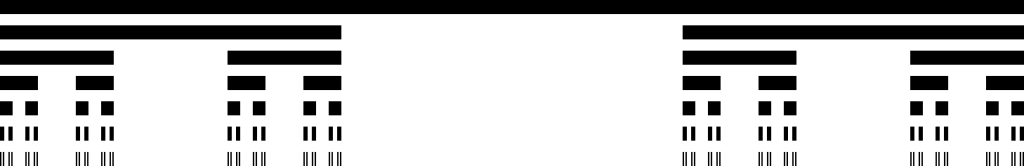
\includegraphics[width=0.8\textwidth]{media/cantor-thirds.png} \\
		\footnotesize Image from \cite{img:cantor}
	\end{center}
	It is a classic fact that $C$ is uncountable
	(it consists of ternary expansions omitting the digit $1$).
	But it is measurable (it is an intersection of closed sets!)
	and we contend it has measure zero.
	Indeed, at the $n$th step, the result has measure $(2/3)^n$ leftover.
	So $\mu(C) \le (2/3)^n$ for every $n$, forcing $\mu(C) = 0$.
\end{example}

This is fantastic, but there is one elephant in the room:
how are the Lebesgue $\sigma$-algebra and the Borel $\sigma$-algebra related?
To answer this question briefly, I will state two results
(but another answer is given in the next section).
The first is a geometric interpretation of the strange
Carath\'{e}odory measurable hypothesis.
\begin{proposition}
	[A geometric interpretation of Lebesgue measurability]
	\label{prop:lebesgue_geo}
	A set $A \subseteq \RR^n$ is Lebesgue measurable
	if and only if for every $\eps > 0$,
	there is an open set $U \supset A$ such that
	\[ \lambda^\ast(U \setminus A) < \eps \]
	where $\lambda^\ast$ is the Lebesgue outer measure.
\end{proposition}
I want to say that this was Lebesgue's original formulation
of ``measurable'', but I'm not sure about that.
In any case, we won't need to use this,
but it's good to see that our definition of Lebesgue measurable
has a down-to-earth geometric interpretation.

\begin{ques}
	Deduce that every open set is Lebesgue measurable.
	Conclude that the Lebesgue $\sigma$-algebra
	contains the Borel $\sigma$-algebra.
	(A different proof is given later on.)
\end{ques}

However, the containment is proper:
there are more Lebesgue measurable sets than Borel ones.
Indeed, it can actually be proven using transfinite induction
(though we won't) that
$\left\lvert \SB(\RR) \right\rvert = \left\lvert \RR \right\rvert$.
Using this, one obtains:
\begin{exercise}
	Show the Borel $\sigma$-algebra is not complete.
	(Hint: consider the Cantor set.
	You won't be able to write down an example of a non-measurable
	set, but you can use cardinality arguments.)
	Thus the Lebesgue $\sigma$-algebra strictly contains the Borel one.
	% It should contain every subset of the Cantor set,
	% since Lebesgue is complete.
\end{exercise}

Nonetheless, there is a great way to describe the Lebesgue $\sigma$-algebra,
using the idea of completeness.
\begin{definition}
	Let $(\Omega, \SA, \mu)$ be a measure space.
	The \vocab{completion} $(\Omega, \ol{\SA}, \ol{\mu})$
	is defined as follows:
	we let
	\[ \ol{\SA} = \left\{ A \cup N \mid A \in \SA,
		N \text{ subset of null set} \right\}. \]
	and $\ol{\mu}(A \cup N) = \mu(A)$.
	One can check this is well-defined,
	and in fact $\ol{\mu}$ is the unique extension
	of $\mu$ from $\SA$ to $\ol{\SA}$.

	This looks more complicated than it is.
	Intuitively, all we are doing is ``completing'' the measure
	by telling $\ol{\mu}$ to regard any subset of a null set
	as having measure zero, too.
\end{definition}

Then, the saving grace:
\begin{theorem}
	[Lebesgue is completion of Borel]
	For $\RR^n$, the Lebesgue measure is the completion of the Borel measure.
\end{theorem}
\begin{proof}
	This actually follows from results in the next section,
	namely \Cref{exer:cubes_vs_open}
	and part (c) of Carath\'{e}odory for pre-measures (\Cref{thm:cara_premeasure}).
\end{proof}

\section{A fourth row: Carath\'{e}odory for pre-measures}
\prototype{The fourth row for the Lebesgue measure is $\SB(\RR^n)$.}
In many cases, $\SA\cme$ is actually bigger than our original goal,
and instead we only need to extend $\mu_0$ on $\SA_0$
to $\mu$ on $\SA$, where $\SA$ is the $\sigma$-algebra generated by $\SA_0$.
Indeed, our original goal was to get $\SB(\RR^n)$, and in fact:
\begin{exercise}
	Show that $\SB(\RR^n)$ is the $\sigma$-algebra generated
	by the $\mathcal{L}_0$ we defined earlier.
	\label{exer:cubes_vs_open}
\end{exercise}

Fortunately, this restriction is trivial to do.
\begin{ques}
	Show that $\SA\cme \supset \SA$,
	so we can just restrict $\mu\cme$ to $\SA$.
\end{ques}
We will in a moment add this as the fourth row in our table.

However, if this is the end goal,
than a somewhat different Carath\'{e}odory theorem
can be stated because often one more niceness condition holds:
\begin{definition}
	A pre-measure or measure $\mu$ on $\Omega$ is \vocab{$\sigma$-finite}
	if $\Omega$ can be written as a countable union $\Omega = \bigcup_n A_n$
	with $\mu(A_n) < \infty$ for each $n$.
\end{definition}
\begin{ques}
	Show that the pre-measure $\lambda_0$ we had,
	as well as the Borel measure $\SB(\RR^n)$,
	are both $\sigma$-finite.
\end{ques}
Actually, for us, $\sigma$-finite is basically always going to be true,
so you can more or less just take it for granted.

\begin{theorem}
	[Carath\'{e}odory extension theorem for pre-measures]
	\label{thm:cara_premeasure}
	Let $\mu_0$ be a pre-measure on an algebra $\SA_0$ of $\Omega$,
	and let $\SA$ denote the $\sigma$-algebra generated by $\SA_0$.
	Let $\SA\cme$, $\mu\cme$ be as in \Cref{thm:cara_outer}.
	Then:
	\begin{enumerate}[(a)]
		\ii The restriction of $\mu\cme$ to $\SA$
		gives a measure $\mu$ extending $\mu_0$.
		\ii If $\mu_0$ was $\sigma$-finite,
		then $\mu$ is the unique extension of $\mu_0$ to $\SA$.
		\ii If $\mu_0$ was $\sigma$-finite,
		then $\mu\cme$ is the completion of $\mu$,
		hence the unique extension of $\mu_0$ to $\SA\cme$.
	\end{enumerate}
\end{theorem}
Here is the updated table, with comments if $\mu_0$ was indeed $\sigma$-finite.
\begin{center}
	\begin{tabular}[h]{llcl}
		& & Construct order & Notes \\ \hline
		$2^\Omega$ & $\mu^\ast$ & Step 2 &
			$\mu^\ast$ is outer measure obtained from $\mu_0$ \\[1em]
		$\SA\cme$ & $\mu\cme$ & Step 3 & $(\SA\cme, \mu\cme)$ is completion $(\SA, \mu)$, \\
		&&& $\SA\cme$ defined as $\mu^\ast$-measurable sets \\[1em]
		$\SA$ & $\mu$ & Step 4 & $\SA$ defined as $\sigma$-alg.\ generated by $\SA_0$ \\[1em]
		$\SA_0$ & $\mu_0$ & Step 1 & $\mu_0$ is a pre-measure
	\end{tabular}
\end{center}
And here is the table for $\Omega = \RR^n$,
with Borel and Lebesgue in it.
\begin{center}
	\begin{tabular}[h]{llcl}
		& & Construct order & Notes \\ \hline
		$2^{\RR^n}$ & $\lambda^\ast$ & Step 2 &
			$\lambda^\ast$ is Lebesgue outer measure \\[1em]
		$\mathcal L(\RR^n)$ & $\lambda$ & Step 3 &
			Lebesgue $\sigma$-algebra, completion of Borel one \\[1em]
		$\SB(\RR^n)$ & $\mu$ & Step 4 &
			Borel $\sigma$-algebra, generated by $\mathcal{L}_0$ \\[1em]
		$\mathcal L_0$ & $\lambda_0$ & Step 1 & Define pre-measure on rectangles
	\end{tabular}
\end{center}

Going down one row of the table corresponds to restriction,
while each of $\mu_0 \to \mu \to \mu\cme$ is a unique extension
when $\mu_0$ is $\sigma$-finite.
\begin{proof}
	[Proof of \Cref{thm:cara_premeasure}]
	For (a): this is just \Cref{thm:construct_outer} and \Cref{thm:cara_outer}
	put together, combined with the observation that $\SA^\ast \supset \SA_0$
	and hence $\SA^\ast \supset \SA$.
	Parts (b) and (c) are more technical, and omitted.
\end{proof}

\section{From now on, we assume the Borel measure}
\todo{explain why}

\section{\problemhead}
\begin{dproblem}
	[Constructing outer measures from arbitrary $\rho$]
	\label{pr:construct_outer_measure}
	For a set $\Omega$,
	let $\mathcal{E}$ be \emph{any} subset of $2^{\Omega}$
	and let $\rho \colon \mathcal{E} \to [0,+\infty]$
	be \emph{any} function.
	Prove that
	\[ \mu^\ast(E) = \inf \left\{ \sum_{n=1}^\infty \rho(E_n) \mid
		E_n \in \mathcal{E}, \;
		E \subseteq \bigcup_{n=1}^\infty E_n \right\} \]
	is an outer measure.
\end{dproblem}

\begin{problem}
	[The insane scientist]
	Let $\Omega = \RR^2$, and let $\mathcal{E}$
	be the set of (non-degenerate) rectangles.
	Let $\rho(E) = 1$ for every rectangle $E \in \mathcal{E}$.
	Ignoring my advice, the insane scientist
	uses $\rho$ to construct an outer measure $\mu^\ast$,
	as in \Cref{pr:construct_outer_measure}.
	\begin{enumerate}[(a)]
		\ii Find $\mu^\ast(S)$ for each subset $S$ of $\RR^2$.
		\ii Which sets are $\mu^\ast$-measurable?
	\end{enumerate}
	You should find that no rectangle is $\mu^\ast$-measurable,
	unsurprisingly foiling the scientist.
	\begin{hint}
		Show that
		\[ \mu^\ast(S) = \begin{cases}
				0 & S = \varnothing \\
				1 & S \text{ bounded and nonempty} \\
				\infty & S \text{ not bounded}.
			\end{cases}
		\]
		This lets you solve (b) readily;
		I think the answer is just unbounded sets,
		$\varnothing$, and one-point sets.
	\end{hint}
\end{problem}

\begin{problem}
	\gim
	A function $f \colon \RR \to \RR$ is continuous.
	Must $f$ be measurable with respect to the Lebesgue measure on $\RR$?
\end{problem}
